\chapter{Monitoring neuronal activity over days during learning} \label{chapter_4}

\section{Introduction}\label{sec:chap4_intro}

Given that changing neuronal activity patterns either cause some instability in information coding or require compensation by a dynamic decoding network, it is important to consider what advantages might arise from these changes. Computational models suggest that an advantage of dynamic neuronal representations could be the flexibility of incorporating new information into the population \citep{Ajemian2013, Rokni2007a}. We therefore tested how existing representations were affected by the learning of a new association. We trained the same mice that had already stably performed the task described above to learn a new association.

\section{Results} \label{sec:chap4_results}

\subsection{Task design for learning a stimulus-action pair} \label{chap4:stim_action}

 We introduced a third possible cue (crosshatch pattern) that required a specific turn at the intersection for the mouse to receive a reward (the turn direction was randomly selected for each mouse) (Figure \ref{fig:7_cues}). After a mouse had learned the novel third trial type, we introduced a fourth cue (triangle pattern) that required the mouse to turn the opposite direction of that required for the third cue (Figure \ref{fig:7_cues} a). Mice learned the novel cue-response associations while maintaining high performance for the original two cue-response associations (Figure \ref{fig:7_cues} b).

\begin{figure}
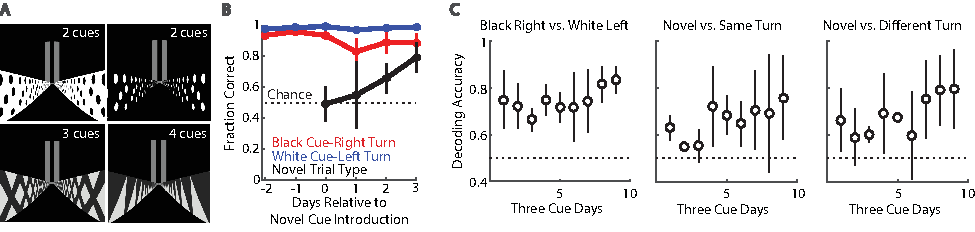
\includegraphics[width=\textwidth]{figures/7_cues.pdf}
\caption[Neuronal activity during learning of a novel trial type]{\textbf{Neuronal activity during learning of a novel trial type a,} Schematic of virtual maze trial types. 
%
\textbf{b,} Behavioral performance on 2 days preceding and 4 days following introduction of a novel trial type. Error bars indicate mean $\pm$ sem. n = 4 (2 mice with 2 novel trial types each).
%
\textbf{c,} Decoding performance of different trial types during the first 1 second of the cue period based on population activity. Error bars indicate mean $\pm$ sem, n = 2 mice. 
\label{fig:7_cues}}
\end{figure}


\subsection{Rate of change during learning compared to stable behavior} \label{chap4:decoding}

We first asked whether the neuronal activity patterns were different between trials in which the mouse saw the novel cues and those in which it saw the familiar cues. Using a decoder based on population activity, the novel trial types were separable from the familiar trial types (Figure \ref{fig:7_cues} c). These differences in activity between trial types could be visualized on a single day based on population activity in a dimensionality-reduced space (Figure \ref{fig:7_pca_all} a). We quantified these differences in the full dimensional space throughout the duration of the task (Figure \ref{fig:7_pca_all} b). We averaged these differences in activity between trial types across sessions for each mouse, again demonstrating the unique population activity that is specific to each mouse. We also quantified differences between trial types using the behavioral data. Interestingly, we found differences in the running patterns of both mice for the same turn that was instructed by a different cue.

\begin{figure}
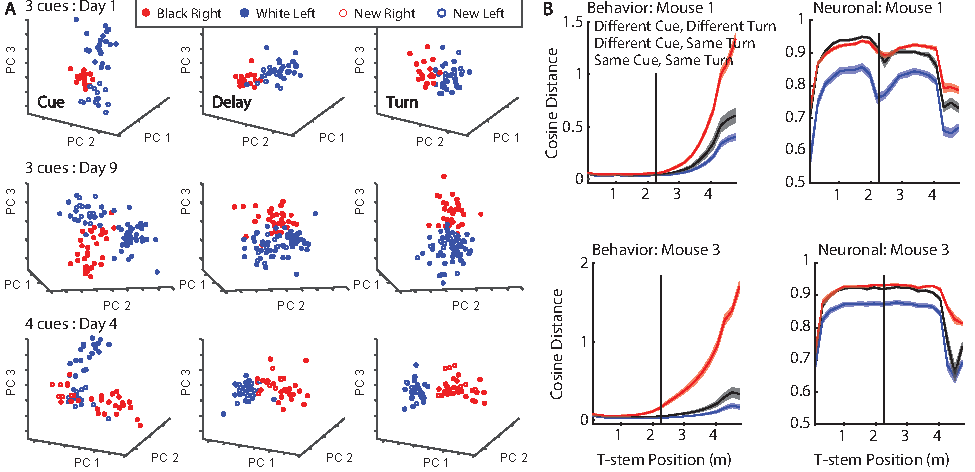
\includegraphics[width=\textwidth]{figures/7_pca_all.pdf}
\caption[Differences in activity between trial types.]{\textbf{Differences in activity between trial types. a,} Cosine distance between single trial population vectors at each of 21 spatial bins spanning the duration of a trial. Cosine distance is computed within a given session for trials with the same cue, different cue but same turn, or different cue and different turn. Error bars indicate mean $\pm$ sem, n = 19 sessions, 1 mouse.
%
\textbf{b,} Example from a single mouse on the final day with four trial types. Top: Population activity during the cue period, delay period, and turn period in the same dimensionality reduced space. Each dot indicates a single trial. 
\label{fig:7_pca_all}}
\end{figure}

We tested if the addition of new learned associations altered the rate at which neuronal activity patterns changed during performance of previously learned trial types. We might expect learning to increase the rate of change as new information is incorporated into network activity. Surprisingly, we found that the rate of change was comparable between the days with stable performance of the two familiar trial types and during learning of the novel trial types (measured based on the performance of models of cells' activity-behavior relationships across days, as in (Figure  \ref{fig:4_glm_across_population}) (Figure \ref{fig:7_rate}).

\begin{figure}
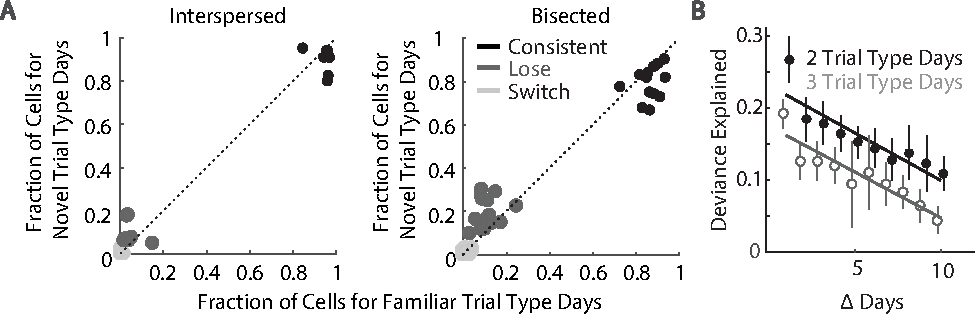
\includegraphics[width=\textwidth]{figures/7_rate.pdf}
\caption[]{\textbf{a,} For interspersed (left panel) and bisected groups (right panel), fraction of cells with, consistent (black), lost (medium gray), switched (light gray) activity-behavior relationships within one session based on our GLM analysis (see methods: GLM encoding model Analysis of model)  on days with two familiar trial types and days with novel trial types. The interspersed group compares models that were built from interspersed chucks throughout the duration of the session and provides us with a baseline for change due to measurement noise. The bisected group compares models that were built from the first and second half of the session.
%
\textbf{b,} For models fit to activity-behavior relationships on one day, the deviance explained of predictions of activity on other days. p = 0.91, ANOVA, comparing linear regression slopes for two trial type and novel trial type days.
\label{fig:7_rate}}
\end{figure}

\subsection{Neurons with novel cue related activity} \label{chap4:novel_cue_pool}

This similar rate of change could have occurred because the cells with activity related to the novel trial types were different from the cells with activity related to familiar trial types. We therefore analyzed if the cells with activity related to novel cues had activity related to familiar cues on previous days. Surprisingly, cells with activity related to novel cues were more likely to come from the group of cells which recently (within the past ten days) had activity related to the familiar cues than from a random sample of neurons (Figure \ref{figures/7_learning_same_pool}). 

\begin{figure}
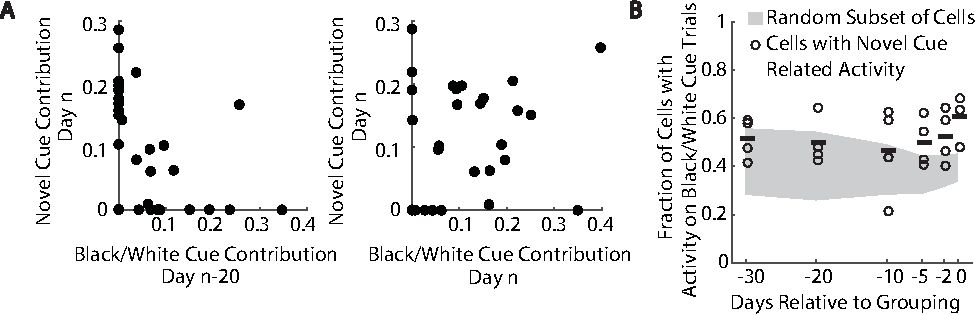
\includegraphics[width=\textwidth]{figures/7_learning_same_pool.pdf}
\caption[Neurons with novel cue related activity came from the pool of cells with recent familiar cue related activity.]{\textbf{Neurons with novel cue related activity came from the pool of cells with recent familiar cue related activity. a,}
Left: For individual cells in mouse 1, novel cue-related activity on day n (measured by > 0 contribution for novel cue onset/offset in the GLM, see Methods) vs. familiar cue-related activity on day n-20. Right: For the same cells, novel cue-related activity on day n vs familiar cue-related activity on day n.
%
\textbf{b,} For cells with novel cue related activity on day n, the fraction of cells with activity related to either white or black cue onset/offset on the same day (day n) and on previous days (days n-2, n-5, n-10, n-20, n-30). Circles indicate individual data points and bars indicate mean, n = 4 (2 mice with 2 novel trial types each). Shaded region indicates 95 $\%$ confidence interval for the fraction of cells with activity on white cue-left turn and black cue-right turn trials taken from a random subset of neurons.
\label{fig:7_learning_same_pool}}
\end{figure}

The evolving pool of cells involved in representing task features was thus more likely to incorporate new task relevant information than the group of cells presently without task relevant information. This finding suggests that new information can be incorporated into the pool of task relevant activity as this pool continuously shifts over time, without disrupting baseline functionality. We speculate that the ability to incorporate new information using 'multitasking' neurons could allow for flexibility during learning, such that the network's ongoing changes provide a framework for the addition of new associations.

\section{Discussion}

We speculate that the changes in neuronal activity reported here reveal key features of how associations are formed and represented in PPC. In particular, our work reveals a potential strategy for a population of neurons to achieve stability in the maintenance of learned associations while also allowing flexibility to incorporate new information.

\bigskip

The rate of reorganization in neuronal activity-behavior relationships was only slightly elevated during learning compared to during stable task performance. We propose that continuous reorganization of representations during stable behavior could endow the network with robustness to perturbations due to injury or learning of additional representations. Through the continuous exploration of parameter space for learned behaviors, the network can sample from the unconstrained space of possible solutions. Flexibility in the representation for a single task could allow the continuous addition of new representations without catastrophic forgetting of previously learned representations. These hypotheses must be tested explicitly in artificial systems. This could be done using an artificial neural network where there is no external controller to turn on and off learning. By continuously updating network connections during learning of a single task, this network could be made robust to change during learning of a second task.

\subsection{Trial-trial variability is stable over learning}
After controlling for behavioral choice, we found that neuronal activity patterns did not stabilize over the course of learning. This result is contradictory to a number of motor learning studies \citep{Peters2014, Ganguly2009}. There are a few possible explanations for these conflicting results. 

\bigskip

Emergence of stable patterns could be an artifact of increasing stereotypy of motor behaviors. \citep{Peters2014} demonstrated that over the course of two weeks during learning of a cued lever press task, lever movements on individual trials became more stereotyped over time. Concurrently the number of movement related neurons went through a period of expansion and followed by contraction resulting in a smaller and more stable population of movement-related neurons towards the end of learning. Similar results have been reported over the course of BMI control learning \citep{Ganguly2009}. Our learning task was designed to control for change in the behavioral readout. By first training mice to report a learned stimulus-action pair with a learned behavioral response (left or right turn) before the acquisition of new stimulus-action relationships, we limit the amount of change in the behavioral response. We did not see a progressively stereotyped motor response over the course of the novel stimulus-action pairing. By closer inspection of the correlation matrices reported in these motor learning studies, it is clear that population responses become more similar during initial phases of learning, as motor responses become more stereotyped. However, after this initial phase of motor response learning, it is unclear whether the responses are completely stabilized or if they simply change at a slower rate. It will be important for future studies to control for behavioral change for the examination of neuronal change over learning.

\bigskip

Alternatively, the timescales over which learning occurs could vary across studies such that it is difficult to compare stabilization of neuronal responses. Our learning task simply requires the animal to match one of two possible actions to each novel stimulus. By learning through trial and error, it is possible for the animal to learn the new stimulus-action pair on a single trial. However, behavioral improvement over days suggests our animals are learning this behavior on a prolonged time scale. We see behavioral improvement over the course of four days during learning. \citep{Peters2014} report learning of their lever press task over a similar time scale; therefore, it seems unlikely that differing timescales for learning could explain differences in the stabilization of neuronal responses over time.

\subsection{Steady number of task related neurons during learning}
 In contrast with previous studies in sensory and motor areas, we found the number of neurons with novel trial related activity to be stable over learning \citep{Poort2015, Peters2014}. Rather, from the very first introduction of the novel cues, there was already a large number of neurons with novel cue related activity. We could decode novel trial types from familiar trial types throughout the duration of the trial using neuronal population activity. Our ability to decode novel trial types was stable over learning, with only a slight rise over ten sessions (not a significant trend). These results suggest that the overrepresentation of familiar trial related activity was possibly transferred to novel cue representations. It will be of great interest in future studies to examine the extent to which familiar task representations can be transferred to the learning of novel tasks and the degree of task similarity required for the constructive transfer of these representations.

\bigskip

All of these measures for learning are likely dependent on task design and the brain region of interest. With newly available recording methods for tracking populations of cells over learning and over the course of stable behavior, it will be important to compare these measures across brain regions and across tasks.

\section{Data analysis methods}

\subsection{Dimensionality reduction of neuronal and behavioral data}
We reduced the dimensionality of single trial data into a space that captured the most variance across trial types and epochs of the trial. We performed principal component analysis (PCA) on averaged population responses across these different conditions. We constructed a data matrix X of size $N_{neurons}$ $\times$ $N_{conditions}$, in which columns corresponded to spatially binned z-scored population response vectors for a given segment of the trial (Figure \ref{fig:7_pca_all} a). The principal components (PCs) of this data matrix were vectors $v_a$ of length $N_{neurons}$ indexed by the number of PCs. For visualization, we then projected single trial data onto the first 3 PCs. 

\bigskip

The motivation for this analysis was to visualize differences in single trial data that corresponded to differences in our conditions of interest. In Figure \ref{fig:7_learning_same_pool} we were interested in the evolving population activity throughout the duration of the trial for different trial types on a single day. Our neuronal data matrix X included 345 neurons identified on a single day and 7 spatial bins evenly spanning the duration of the trial for all 4 trial types (28 conditions). We projected single trial data onto the first 3 PCs of this matrix from individual spatial bins 1, 4 and 7 in the cue period, delay period and turn period. This analysis was solely for visualization. All quantified decoding was performed in the full dimensional space. 

\subsection{Cosine distance}
Neuronal cosine distance was calculated from normalized population response vectors of all neurons that were identified on the session of interest (1 spatial bin $\times$ $N_{neurons}$). Behavioral cosine distance was calculated from normalized behavioral variable vectors (translational treadmill velocity, rotational treadmill velocity, view angle) (1 spatial bin $\times$ 3 features). 
